\documentclass[11pt]{article}

\usepackage[margin=1in]{geometry}
\usepackage{amsmath,amssymb,amsfonts}
\usepackage{graphicx}
\usepackage{booktabs}
\usepackage{hyperref}
\usepackage{xcolor}
\usepackage{caption}
\usepackage{subcaption}

\graphicspath{{../code/figs/}}

\newcommand{\vxi}{\boldsymbol{\xi}}
\newcommand{\mhat}[1]{\hat{\mathbf{#1}}}
\newcommand{\R}{\mathbb{R}}
\newcommand{\norm}[1]{\left\lVert #1 \right\rVert}

\title{Supplementary Information:\\
Validated Synthetic Patient Generation for Small Longitudinal Cohorts}
\author{}
\date{}

\begin{document}
\maketitle

\renewcommand{\thefigure}{S\arabic{figure}}
\renewcommand{\thetable}{S\arabic{table}}
\setcounter{figure}{0}
\setcounter{table}{0}

% ══════════════════════════════════════════════════════════════════════════════
\section*{Supplementary Figures}

% ── Level 2 supplement ──────────────────────────────────────────────────────
\begin{figure}[ht]
\centering
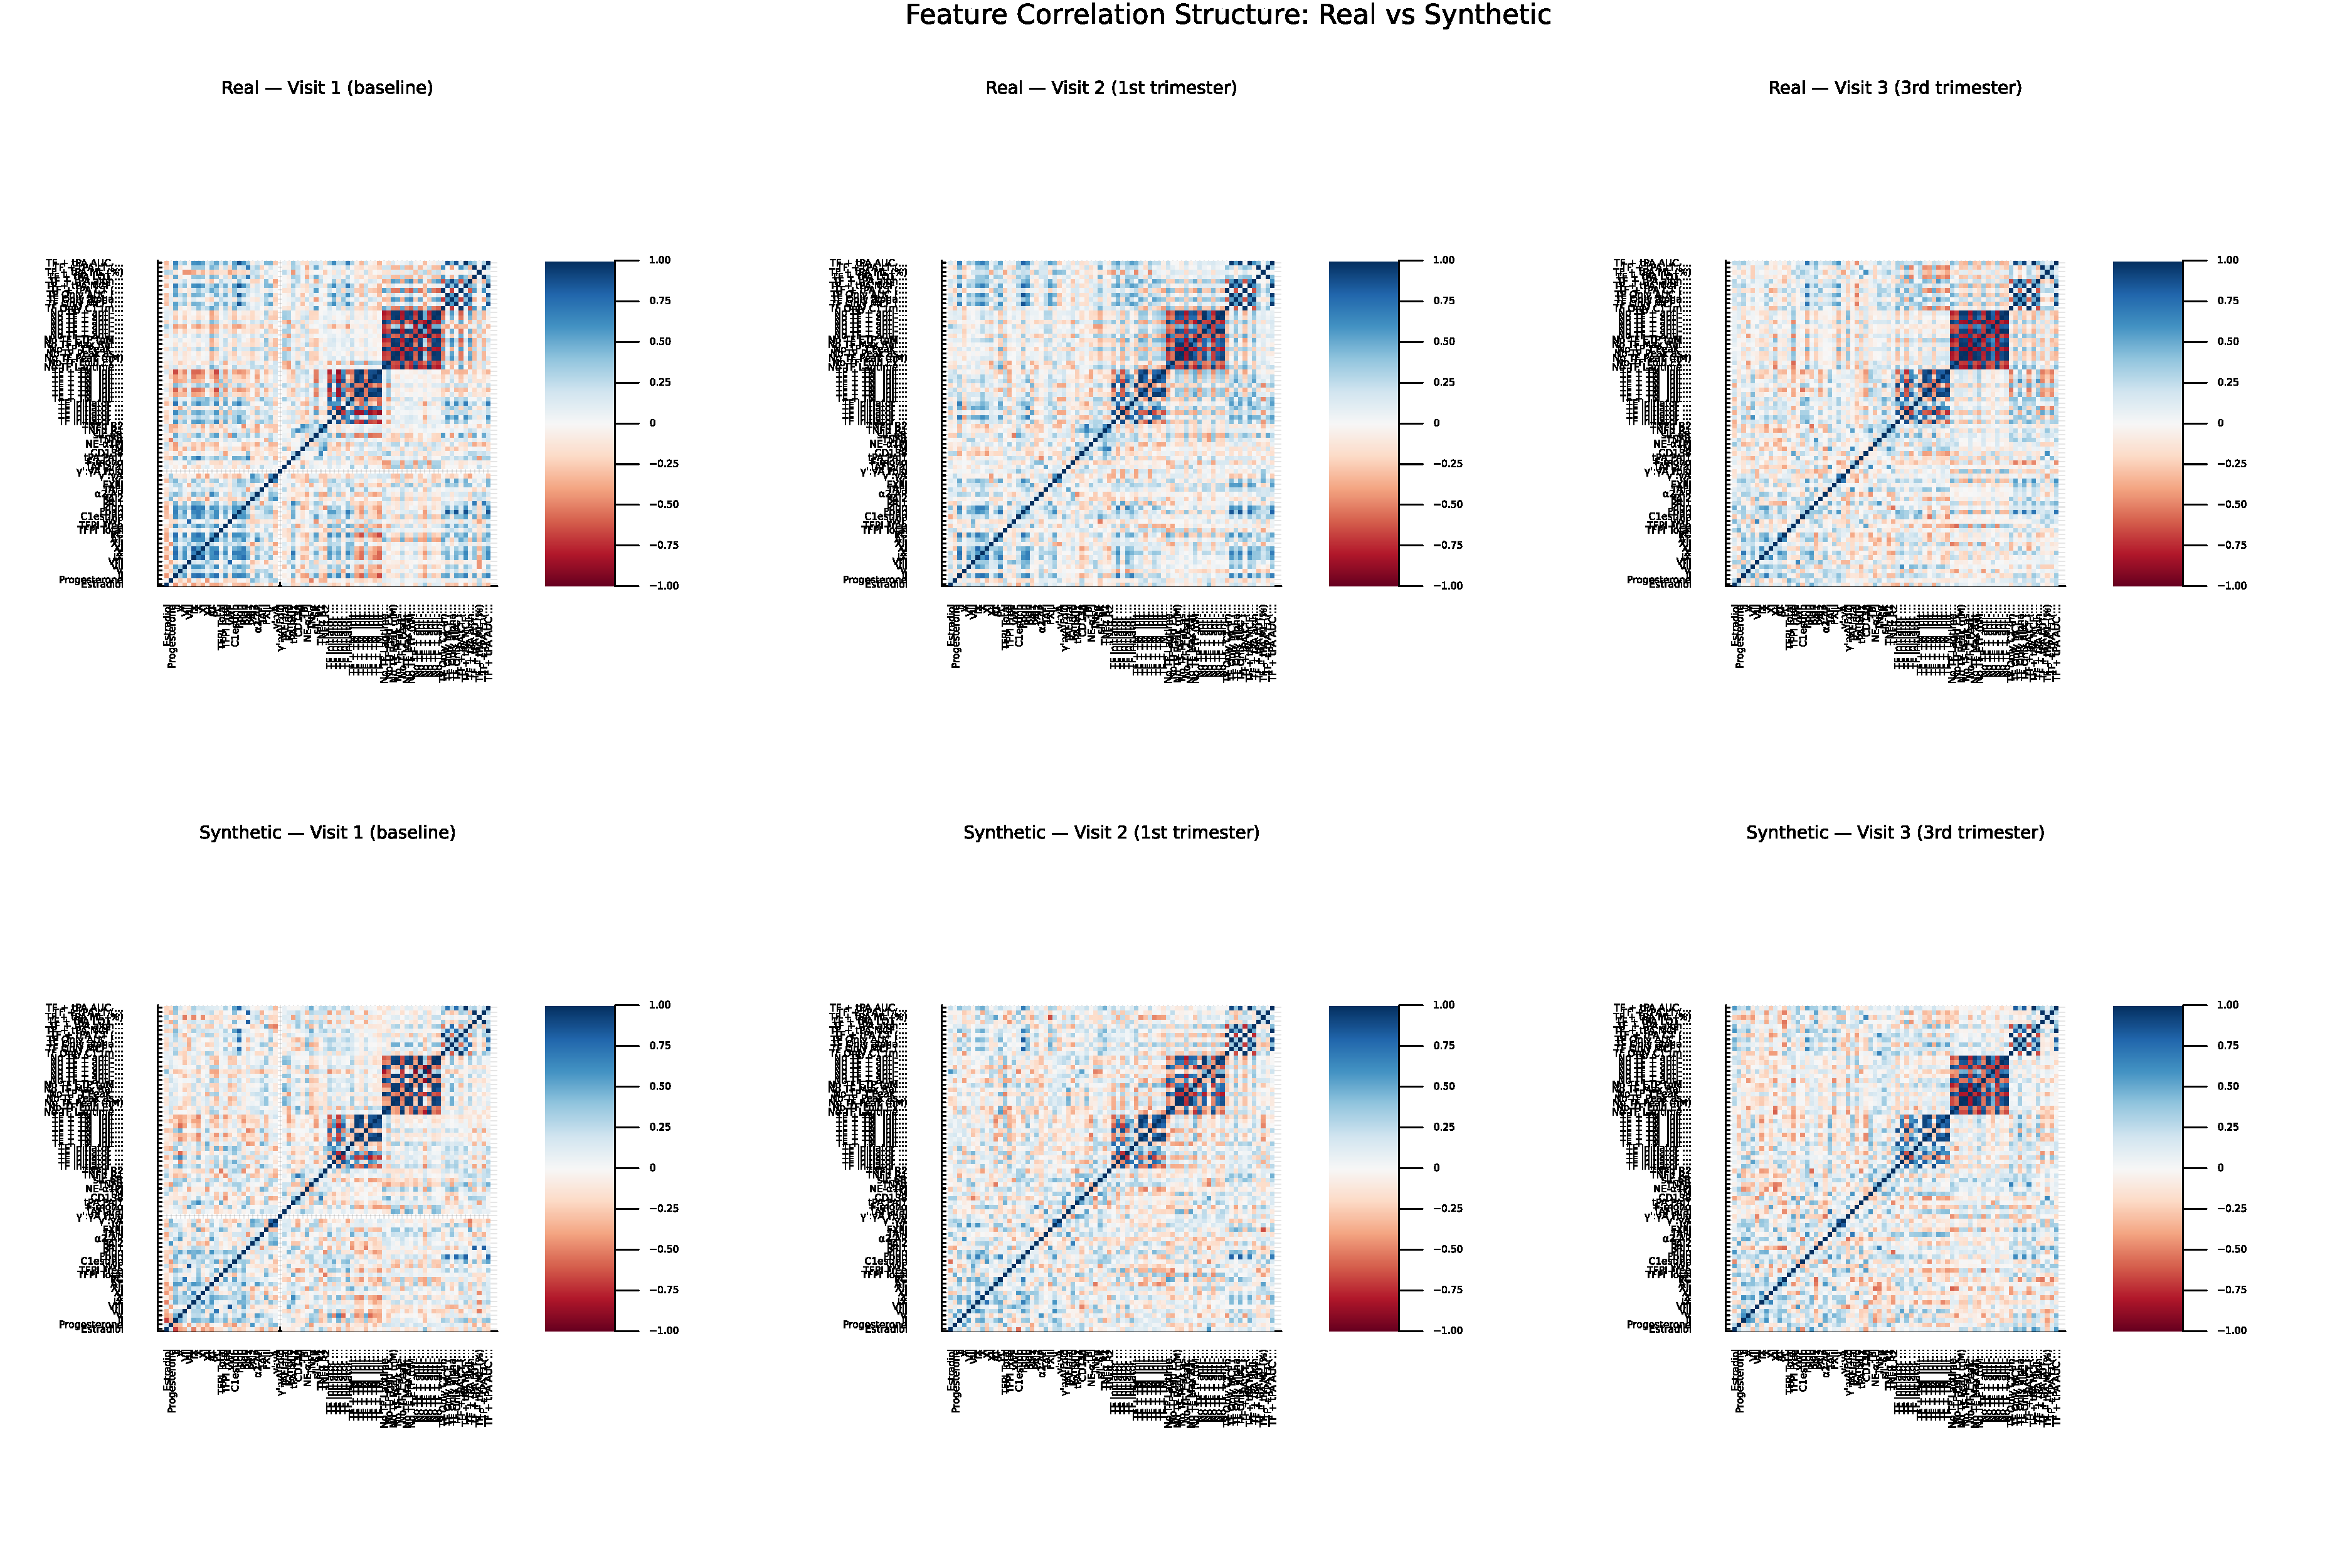
\includegraphics[width=\textwidth]{correlation_heatmaps_paper.pdf}
\caption{\textbf{Within-visit correlation heatmaps.} Pearson correlation matrices
for real and SA-generated synthetic patients within each visit (72 features per
visit). SA preserves the within-visit correlation structure across all three visits.}
\label{sfig:corr-heatmaps}
\end{figure}

\begin{figure}[ht]
\centering
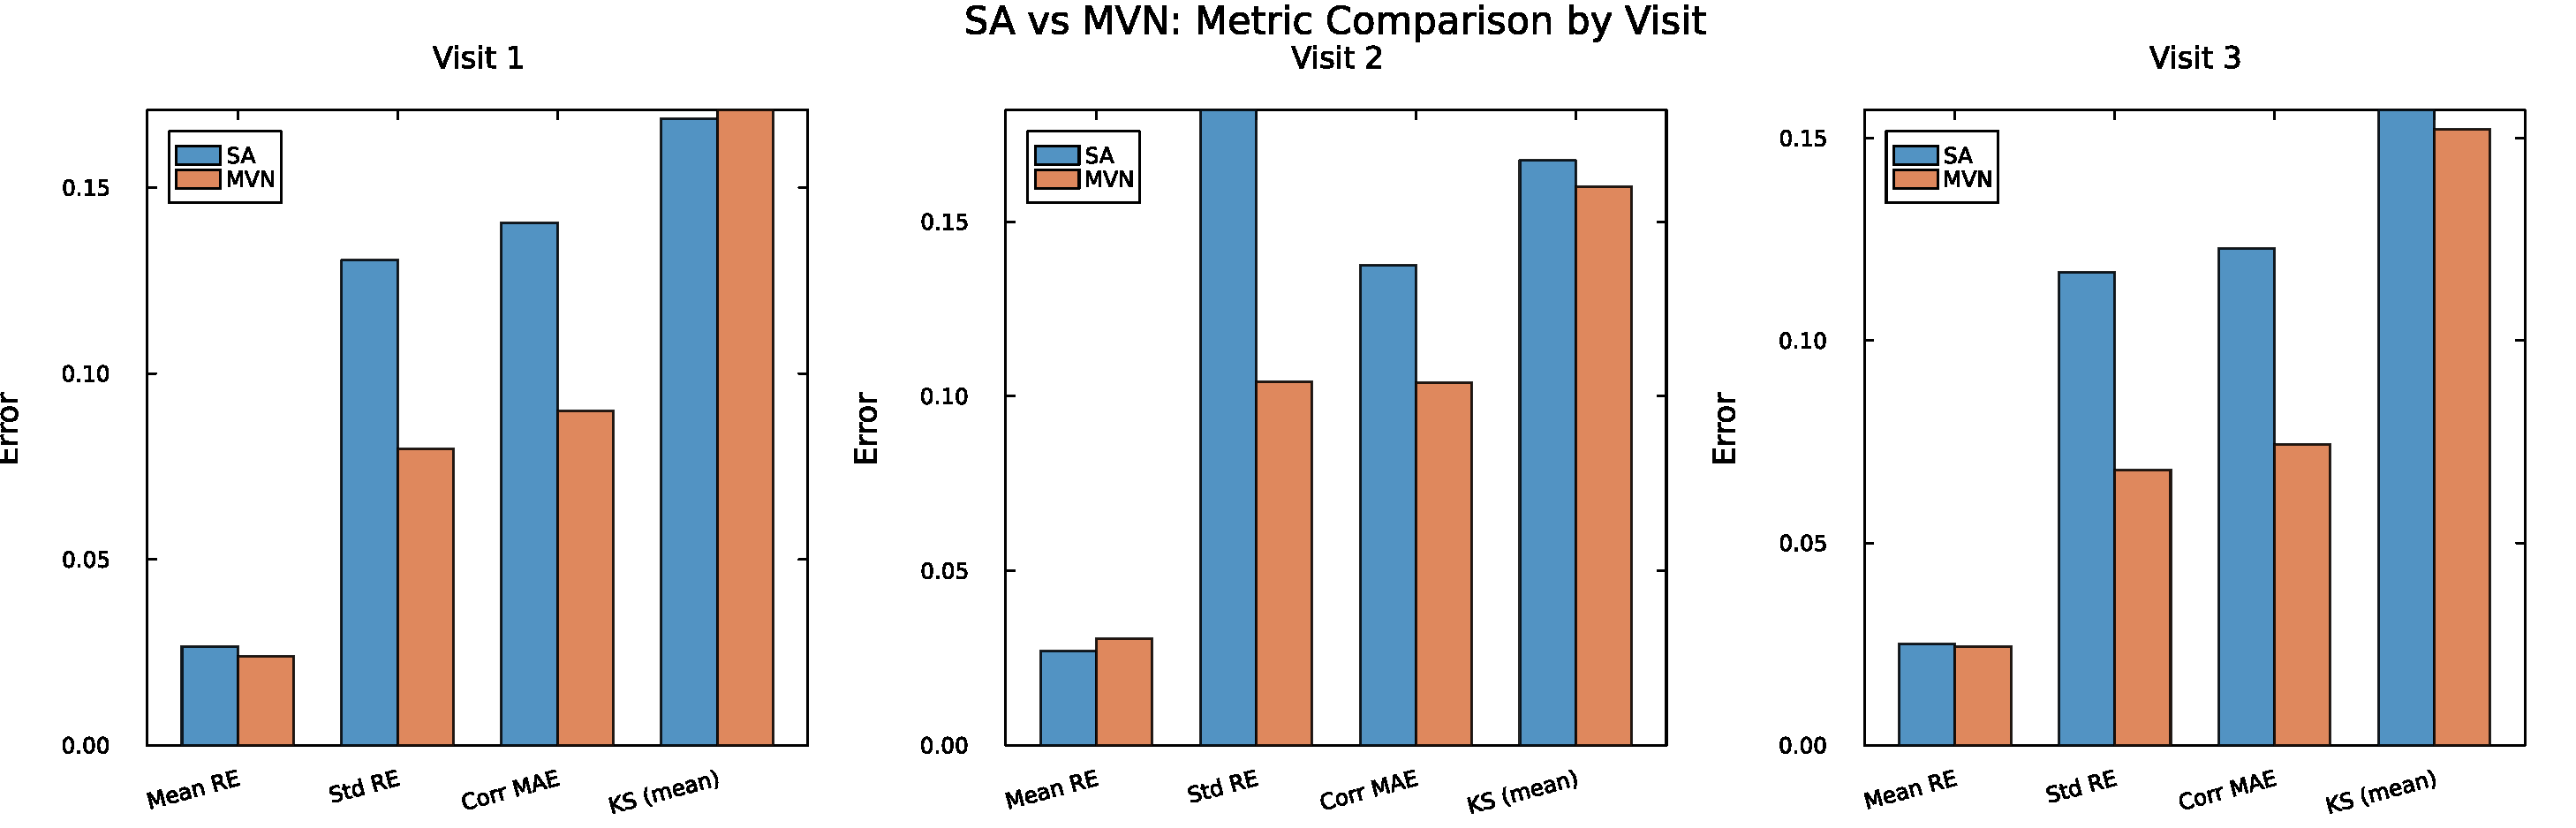
\includegraphics[width=0.7\textwidth]{sa_vs_mvn_metrics_bar.pdf}
\caption{\textbf{SA vs.\ MVN quantitative comparison.} Per-visit comparison of
mean relative error, standard deviation relative error, KS statistic, and
correlation MAE between SA and MVN generation methods. Both methods perform
comparably on marginal statistics (Level~1), but diverge on structural
measures (correlation MAE).}
\label{sfig:metrics-bar}
\end{figure}

% ── Level 3 supplement ──────────────────────────────────────────────────────
\begin{figure}[ht]
\centering
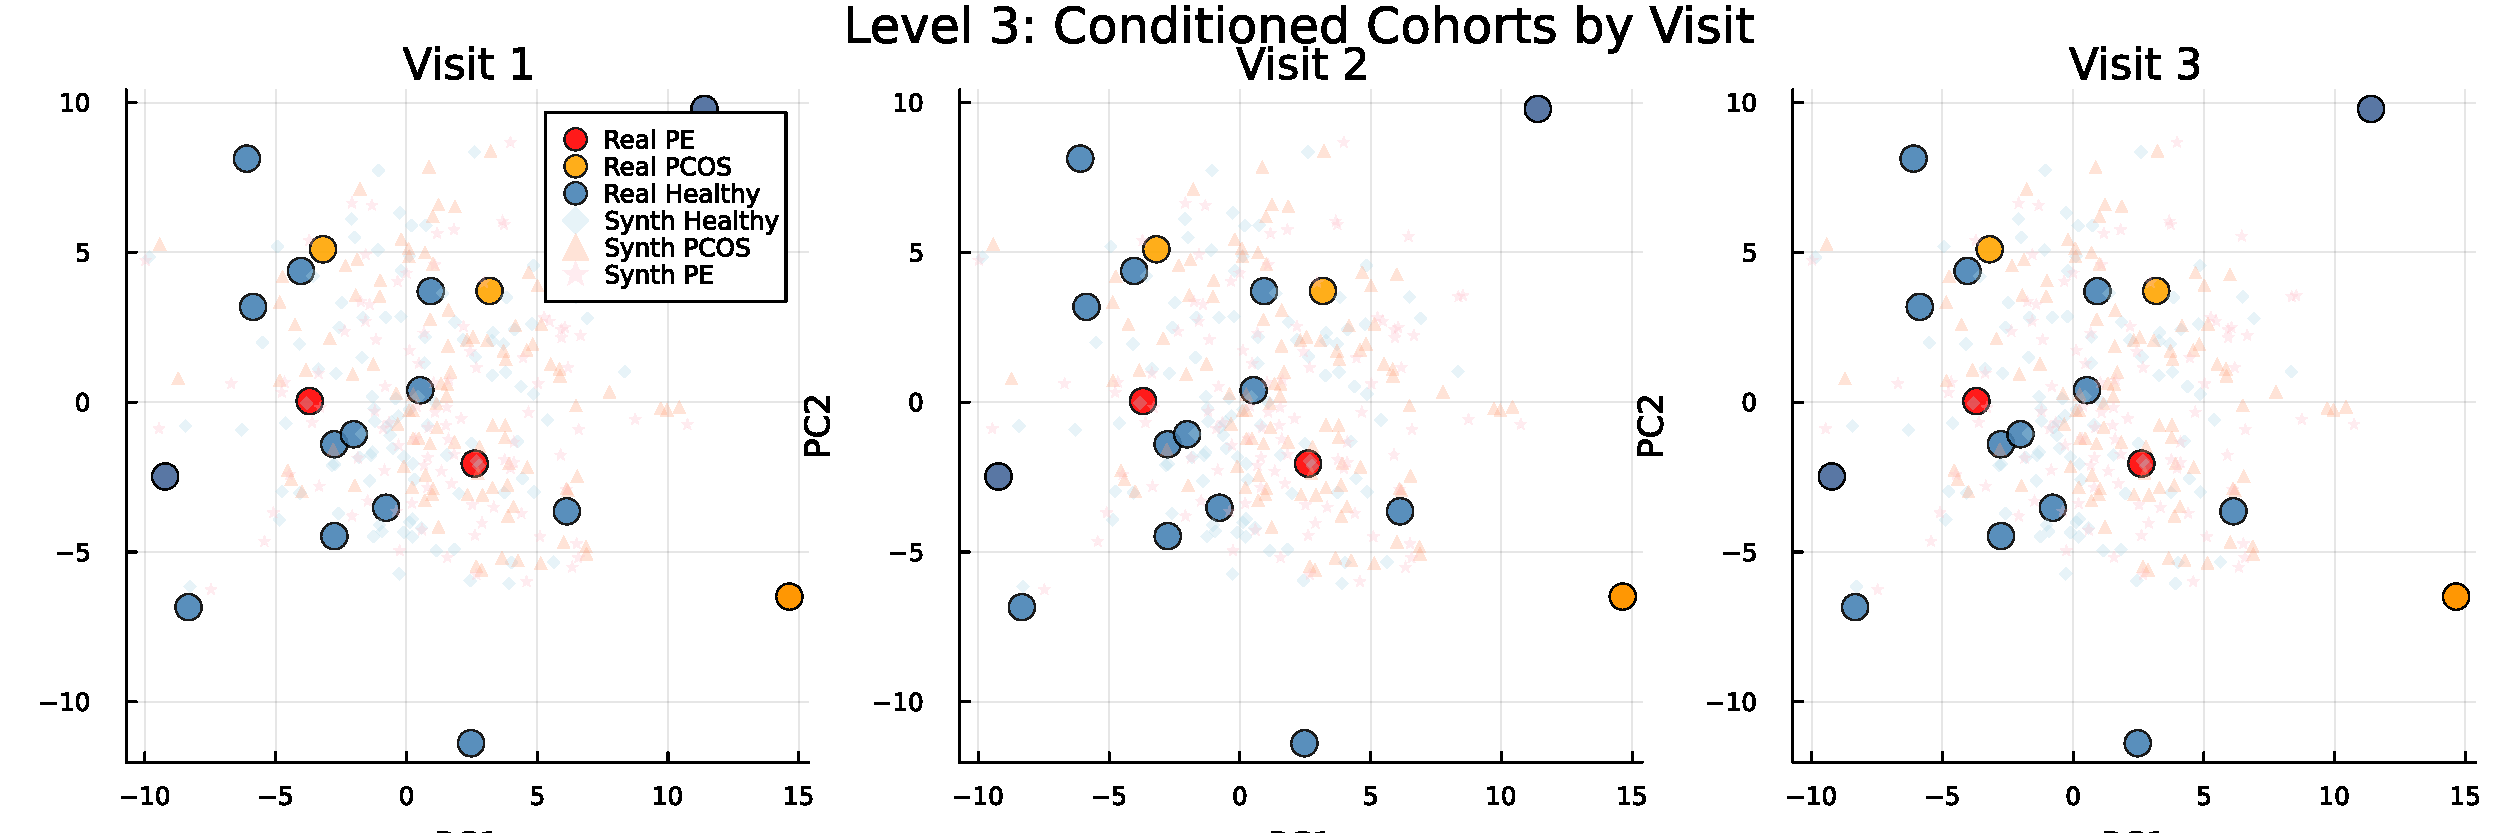
\includegraphics[width=\textwidth]{validate_conditioned_pca_by_visit.pdf}
\caption{\textbf{Conditioned generation by visit.} PCA projections of
condition-specific synthetic cohorts (Healthy, PCOS, PE) separated by visit
(V1, V2, V3). The condition-specific clustering observed in the pooled
projection (Fig.~5 in main text) is maintained within each individual visit.}
\label{sfig:conditioned-by-visit}
\end{figure}

% ── Level 4 supplement ──────────────────────────────────────────────────────
\begin{figure}[ht]
\centering
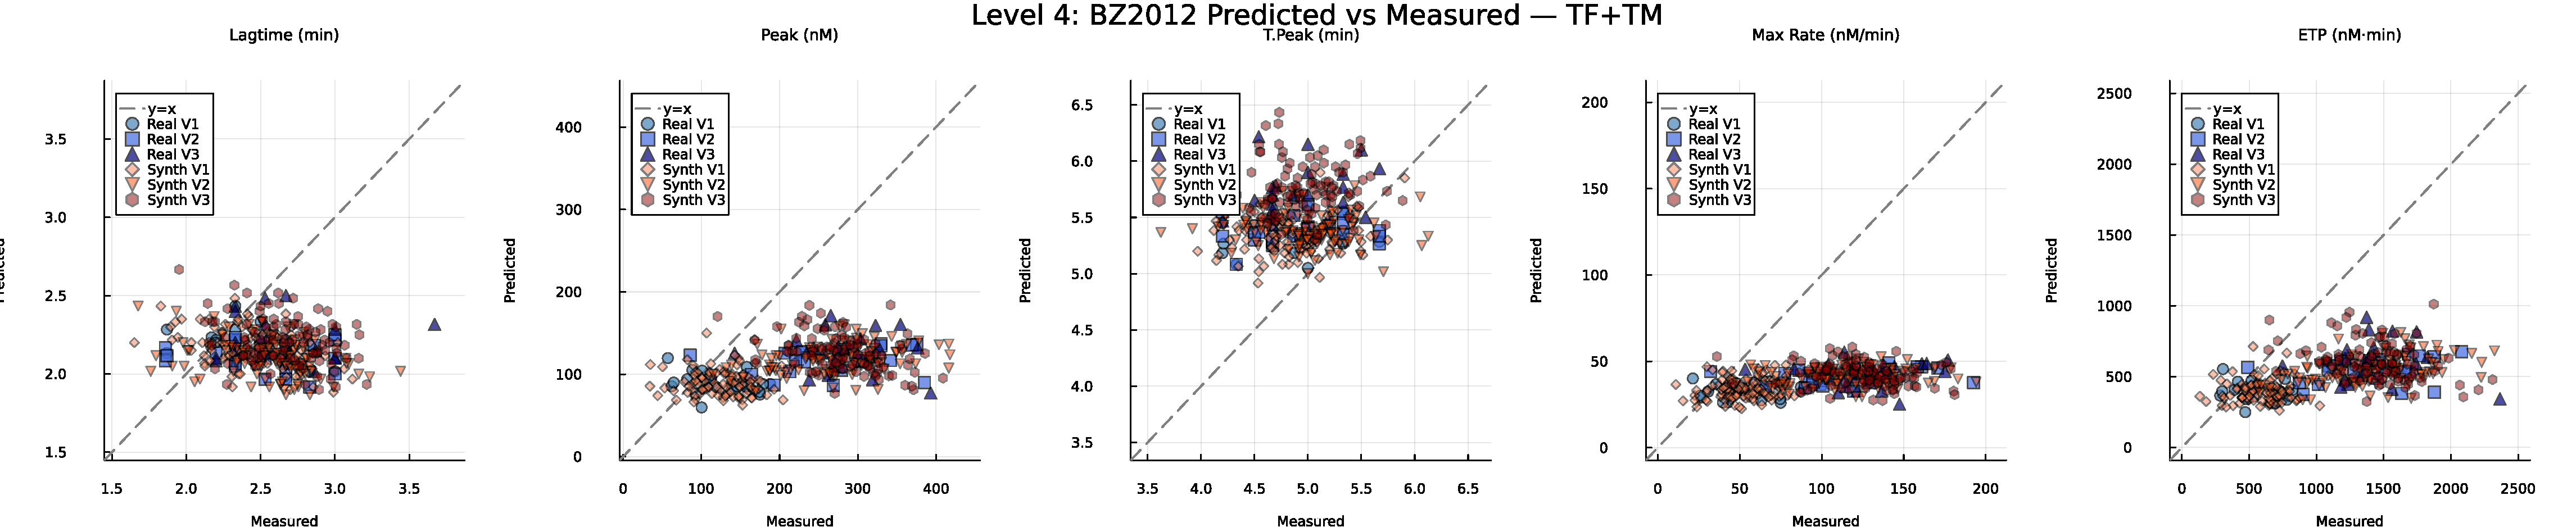
\includegraphics[width=\textwidth]{validate_mechanistic_tf_tm.pdf}
\caption{\textbf{Level~4: Mechanistic model predicted vs.\ measured TGA features
(TF+TM condition).} Same layout as Fig.~6 in the main text. The model
systematically underpredicts peak and maximum rate ($\approx 0.5\times$
measured) for both real and synthetic patients, reflecting overcorrection of
the protein~C anticoagulant pathway. The shared bias indicates that synthetic
patients are processed identically to real patients by the mechanistic model.}
\label{sfig:mechanistic-tm}
\end{figure}

\begin{figure}[ht]
\centering
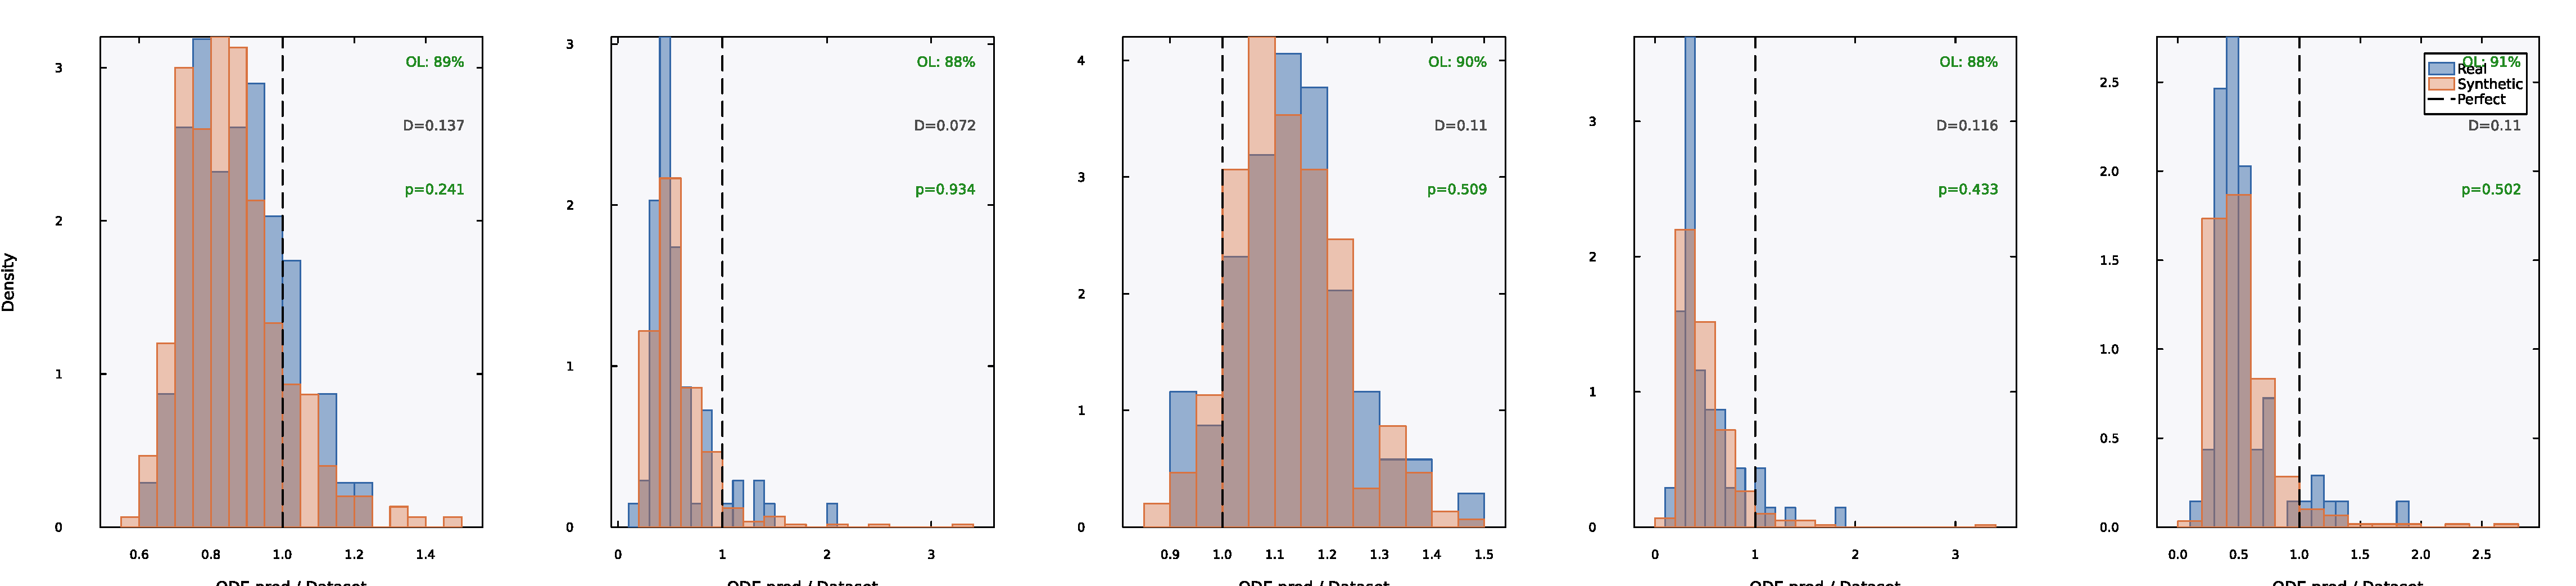
\includegraphics[width=\textwidth]{validate_mechanistic_ratios_tf_tm.pdf}
\caption{\textbf{Level~4: Predicted/measured ratio distributions (TF+TM condition).}
Same layout as Fig.~7 in the main text. Despite the systematic bias in peak
and maximum rate, the ratio distributions for real and synthetic patients
overlap substantially (88--91\% cloud overlap).}
\label{sfig:ratios-tm}
\end{figure}

\begin{figure}[ht]
\centering

\includegraphics[width=\textwidth]{validate_mechanistic_generalization_tf_only.pdf}
\caption{\textbf{Level~4: Cross-visit calibration generalization (TF-only).}
Boxplots of the predicted/measured ratio by visit for real patients. The model
was calibrated on Visit~1 (``train'') only. Ratios near 1.0 at Visits~2 and~3
indicate that the population-level calibration generalizes across pregnancy
timepoints.}
\label{sfig:generalization}
\end{figure}

\begin{figure}[ht]
\centering

\includegraphics[width=0.7\textwidth]{validate_mechanistic_rankcorr_tf_only.pdf}
\caption{\textbf{Level~4: Spearman rank correlations (TF-only).} Mean Spearman
$\rho$ between predicted and measured TGA features, averaged across visits,
for real and synthetic patients. ETP is the best-predicted feature
($\rho \approx 0.6$--$0.8$). Weak rank correlations for other features are
expected given the population-level (not patient-level) calibration.}
\label{sfig:rankcorr}
\end{figure}

\begin{figure}[ht]
\centering

\includegraphics[width=\textwidth]{validate_mechanistic_generalization_tf_tm.pdf}
\caption{\textbf{Level~4: Cross-visit calibration generalization (TF+TM).}
Same layout as Supplementary Fig.~\ref{sfig:generalization}. The TF+TM
calibration does not generalize as well as TF-only, particularly for peak
and maximum rate, due to overcorrection of the protein~C pathway.}
\label{sfig:generalization-tm}
\end{figure}

\begin{figure}[ht]
\centering

\includegraphics[width=0.7\textwidth]{validate_mechanistic_rankcorr_tf_tm.pdf}
\caption{\textbf{Level~4: Spearman rank correlations (TF+TM).} Same layout as
Supplementary Fig.~\ref{sfig:rankcorr}. Rank correlations under TF+TM are
generally weaker than TF-only, consistent with the poorer calibration
generalization under this condition.}
\label{sfig:rankcorr-tm}
\end{figure}

% ── Additional figures ──────────────────────────────────────────────────────
\begin{figure}[ht]
\centering
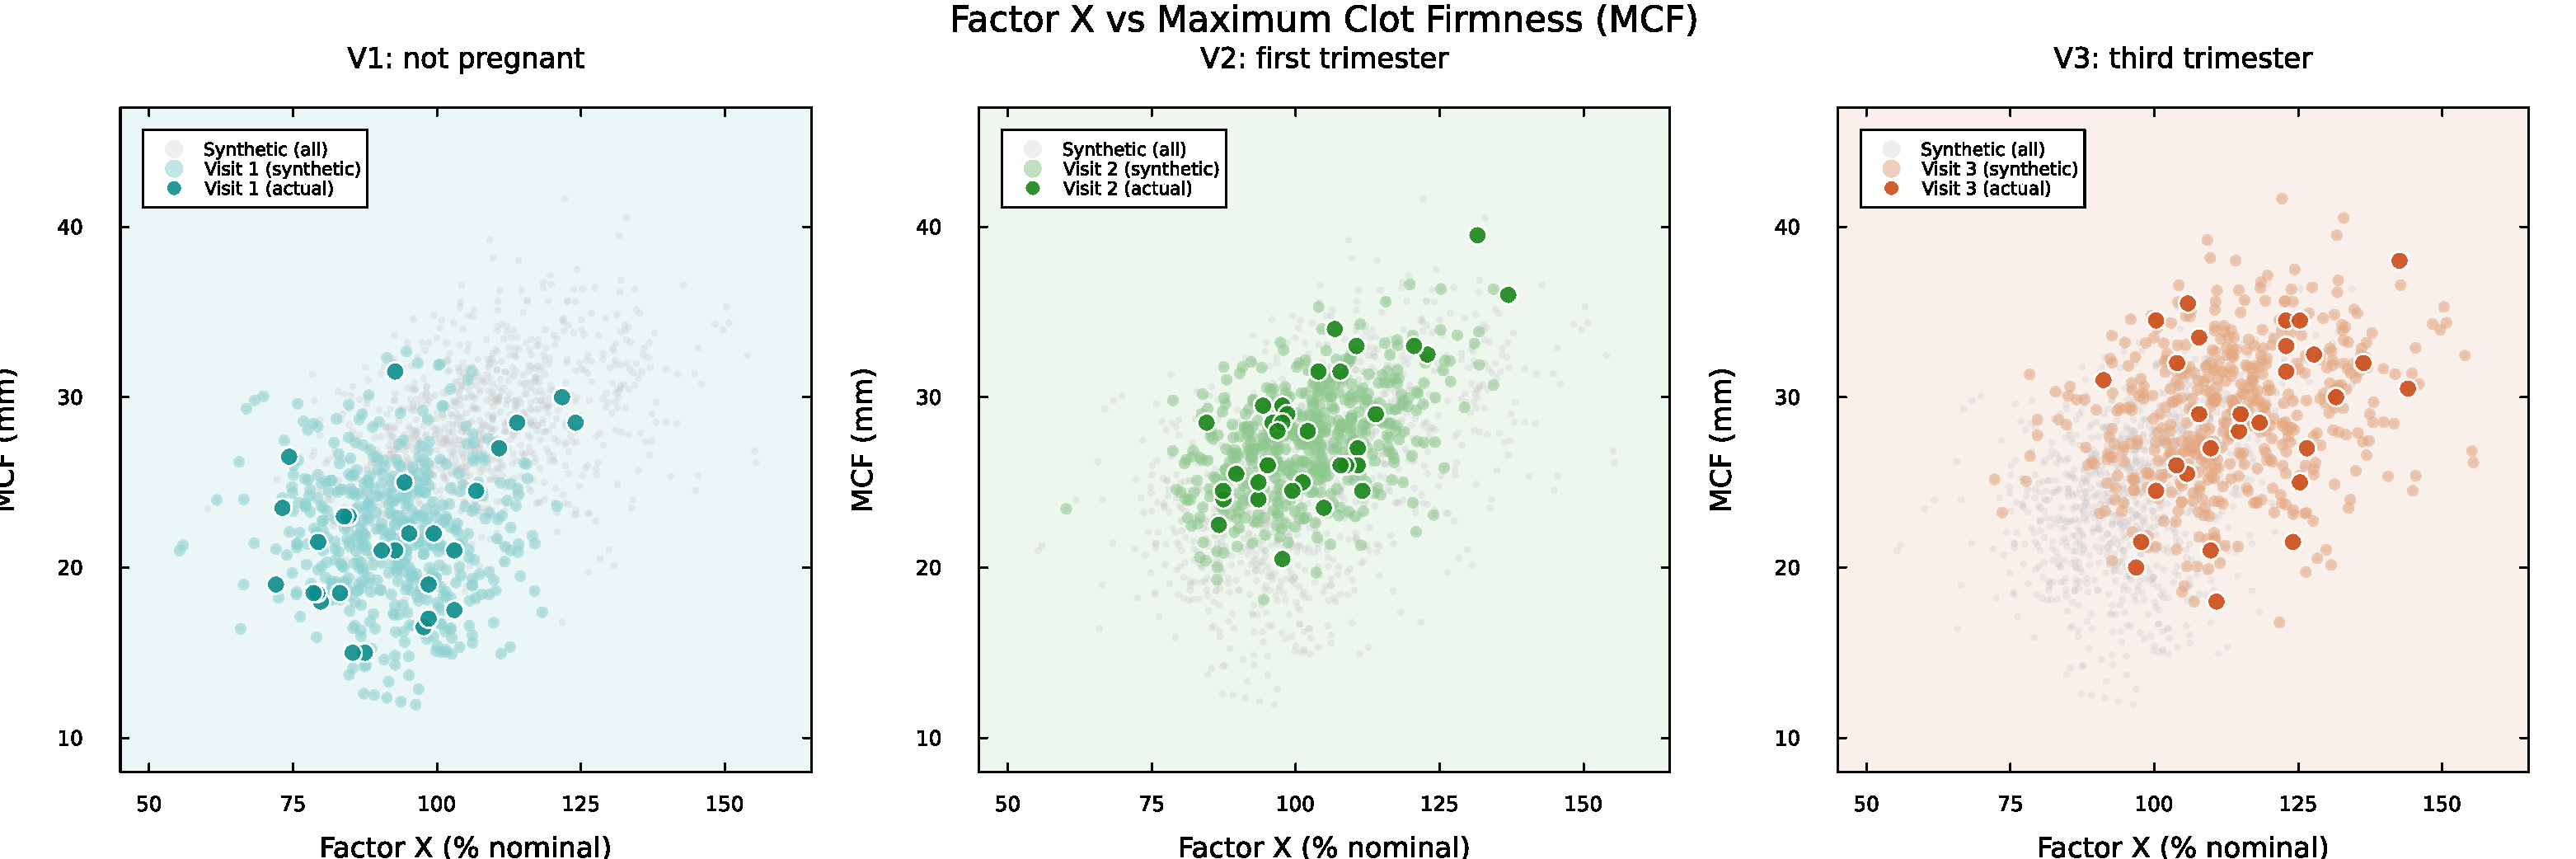
\includegraphics[width=\textwidth]{X_vs_MCF_paper.pdf}
\caption{\textbf{Factor~X vs.\ Maximum Clot Firmness (MCF) trajectory.}
The characteristic pregnancy-driven shift in the Factor~X--MCF plane is
preserved in SA-generated synthetic patients, demonstrating that biologically
meaningful multivariate trajectories are captured by the generation pipeline.}
\label{sfig:x-vs-mcf}
\end{figure}

\begin{figure}[ht]
\centering
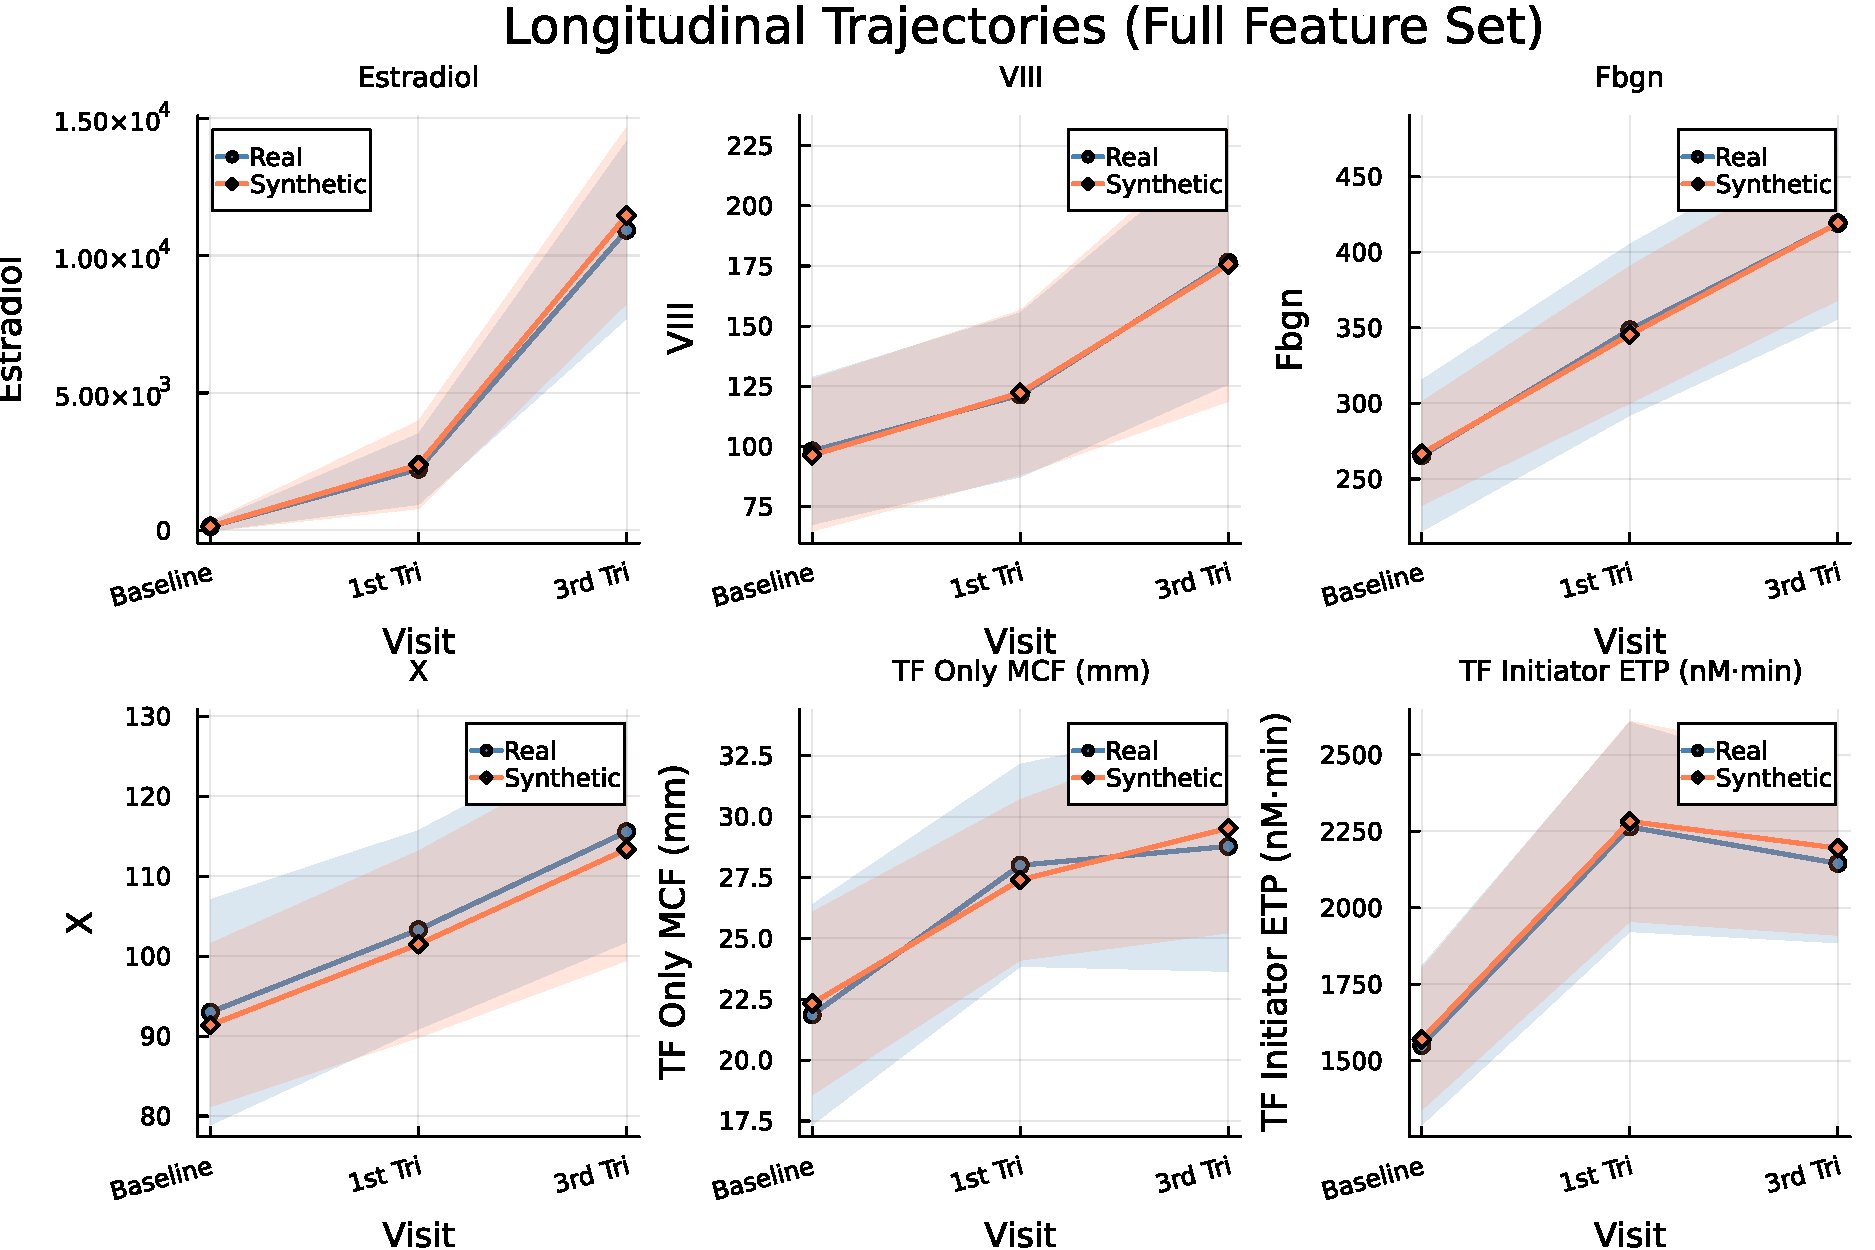
\includegraphics[width=\textwidth]{full_longitudinal_trajectories.pdf}
\caption{\textbf{Full longitudinal trajectories.} Individual patient trajectories
(all 72 features) across three visits for both real and SA-generated synthetic
patients, demonstrating coherent longitudinal patterns.}
\label{sfig:full-trajectories}
\end{figure}

\end{document}
